\documentclass{article}
\usepackage{graphicx}
\newcommand{\code}[1]{\texttt{#1}}
\title{Slurm simulations for investigating Fair Share settings}
\author{Dustin Lang}
\date{\today}
\begin{document}
\maketitle

\section{Simulation}

I wrote a simple notebook (\code{slurm-sim.ipynb}) that tries to reproduce the fair-share and priority queuing
algorithms we have running on Symmetry.

In this simulation, I'm assuming every job takes exactly one hour and
uses a single node.  We'll simulate a case where one user has a lot of
jobs queued, and then, after a week, another user submits a bunch of
jobs.  Specifically: User 1 has submitted enough jobs to keep the
whole cluster for 2 weeks.  Then, after 1 week, User 2 submits enough
jobs to keep the cluster busy for a week.

\paragraph{Configuration settings}
Currently, on Symmetry we use the \code{Priority/multifactor} plugin
to compute job priorities.  The way we have it configured, a job's
priority is the weighted sum of an Age factor (how long the job has
been queued) and a Fair-share factor (which is large if the user has
not been using the cluster, and decreases as the user uses more and
more compute time).  The Age and Fair-share factors are each between 0
and 1.

Parameters:
\begin{description}
  \item[\code{PriorityMaxAge = 10-0}] This settings (10 days)
    determines how long it takes the Age priority factor to go from
    0.0 to 1.0.  That is, the Age priority factor increases by 0.1
    each day, up to a max of ten days.
  \item[\code{PriorityDecayHalflife = 7-0}] This setting determines
    how quickly a user's past usage is ignored in computing the
    Fair-share factor.
  \item[\code{FairShareDampeningFactor = 20}] The Fair-share
    algorithm computes a user's CPU use relative to what you would
    get if you split the cluster evenly between the total number of
    users.  On Symmetry, we have over 150 user accounts, but usually
    only a handful of people active at any time, so the default
    makes a user's fair share tiny.  This factor corrects for that,
    effectively scaling each user's even share up by this factor.
  \item[\code{PriorityWeightAge = 10000}] This determines how much the
    Age factor is scaled to compute the priority.  A larger value
    makes Age (time in queue) more important.
  \item[\code{PriorityWeightFairShare = 4000}] This determines how
    much the Fair-share factor is scaled to compute the priority.  A
    larger value makes a user's past cluster (over)use more important.
\end{description}

\subsection{Run 1}
The first run is with the current values as given above.

Figure \ref{fig:one-age} below shows the Age factor for each user's
jobs.  Recall that User 1 submits a bunch of jobs a time 0, and User 2
submits a bunch of jobs after 1 week.  Each user's jobs gain Age
priority as time goes on, up to the max after 10 days.
\begin{figure}[h!]
  \begin{center}
    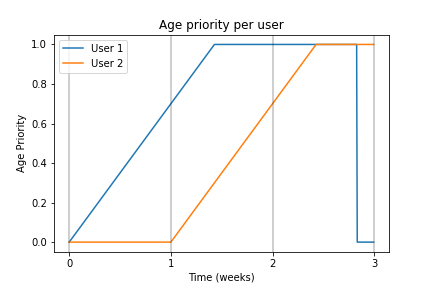
\includegraphics[width=0.8\textwidth]{sim-1-age}
  \end{center}
  \caption{Run 1: Maximum Age factor for jobs submitted by each user.
    \label{fig:one-age}}
\end{figure}

\newpage

Figure \ref{fig:one-fs} below shows the Fair-share factor for each
user.  If the user has not had any jobs running, that user's
Fair-share factor will be 1, and as the user dominates the cluster
over time, it drops to zero.  Here, we see that as User 1 is using the
entire cluster for the first week, the Fair-share factor drops quickly
toward zero.  Once User 2's jobs start running, that user's Fair-share
also drops.
\begin{figure}[h!]
  \begin{center}
    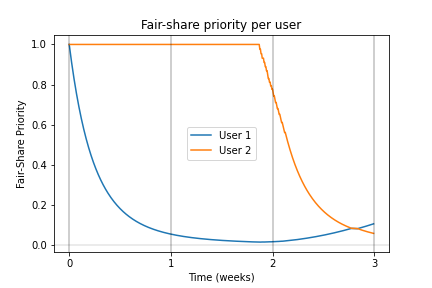
\includegraphics[width=0.8\textwidth]{sim-1-fairshare}
  \end{center}
  \caption{Run 1: Fair-share factor for each user.
    \label{fig:one-fs}}
\end{figure}
\newpage
Figure \ref{fig:one-prio} below shows the total priority: a weighted
sum of the Age factor and Fair-share factor.  At the end of the first
week, User 1's Age priority has reached $0.7 \times 10,000$, and
Fair-share priority is small.  User 2's jobs then begin with no Age
priority and the maximum Fair-share priority, which, because of the
relatively smaller weighting, gives a smaller total weighting of only
$4000$.  Over the next three days, User 1 continues to get all the
compute time, until that user's jobs hit the 10-day max for
accumulating Age priority.  Then User 2's jobs continue accumulating
Age priority, eventually catching up the $\sim3000$-point gap over
about three days.  On day $\sim6$, User 2's jobs finally start running.
\begin{figure}[h!!]
  \begin{center}
    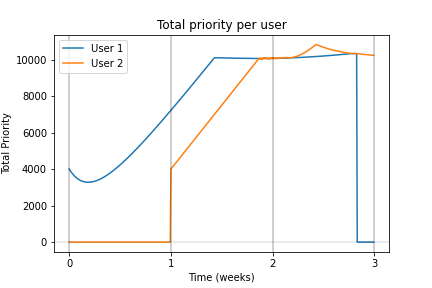
\includegraphics[width=0.8\textwidth]{sim-1-prio}
  \end{center}
  \caption{Run 1: Total priority for each user's jobs.
    \label{fig:one-prio}}
\end{figure}

\clearpage
Figure \ref{fig:one-jobs} shows the scheduler's behaviour.  As
mentioned above, User 1's jobs continue to get scheduled until nearly
a full week after User 2's jobs are submitted.
\begin{figure}[h!]
  \begin{center}
    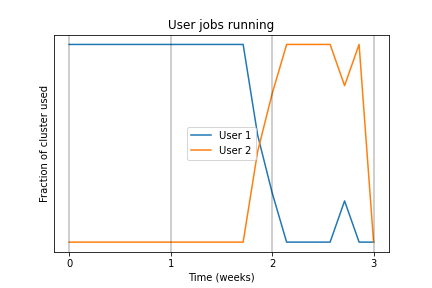
\includegraphics[width=0.8\textwidth]{sim-1-ujobs}
  \end{center}
  \caption{Run 1: Scheduler behaviour: which user's jobs were run over time.
    \label{fig:one-jobs}}
\end{figure}

\clearpage
\subsection{Run 2}
It seems that our weighting of the Fair-share factor is too small
relative to the Age factor.  In this run, we set
\code{PriorityWeightFairShare = 10000}.

The Age factor plot is exactly the same as before.  The Fair-share
factor is similar; we will show it later.  The driving change here is
the total priority, shown below in Figure \ref{fig:two-prio}.  Now,
when User 2's jobs are submitted at the 1-week mark, that user's
Fair-share factor of 1, times the increased weight factor of $10,000$,
is enough for it to beat the priority accumulated by User 1's long
wait.  User 2's jobs begin to run immediately.  However, when that
happens, User 2's Fair-share drops quickly, until its priority drops
below that of User 1.  Then, both users' jobs are run, which reduces
their Fair-shares respectively.  Since User 2 is in a steeper portion
of the Fair-share curve, that user gets a relatively smaller share of
the cluster.

At the 10-day mark, the dynamics change again, because User 1's jobs
stop accumulating Age priority, and User 2 starts getting a larger
share of the cluster.

\begin{figure}[h!!]
  \begin{center}
    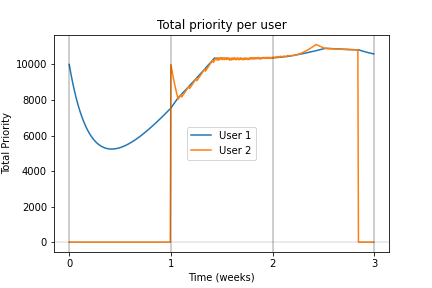
\includegraphics[width=0.8\textwidth]{sim-2-prio}
  \end{center}
  \caption{Run 2: Total priority for each user's jobs.
    \label{fig:two-prio}}
\end{figure}

\clearpage
Figure \ref{fig:two-jobs} shows the jobs run for each user.
As discussed above, the dynamics are surprisingly complicated!
\begin{figure}[h!]
  \begin{center}
    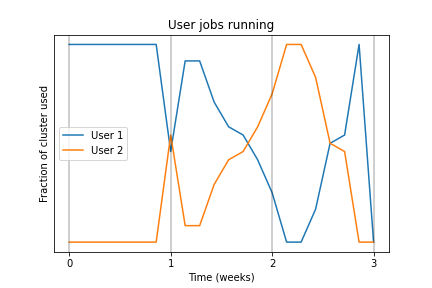
\includegraphics[width=0.8\textwidth]{sim-2-ujobs}
  \end{center}
  \caption{Run 2: Scheduler behaviour: which user's jobs were run over time.
    \label{fig:two-jobs}}
\end{figure}

For completeness, Figure \ref{fig:two-fs} shows the Fair-share
factor for each user.
\begin{figure}[h!]
  \begin{center}
    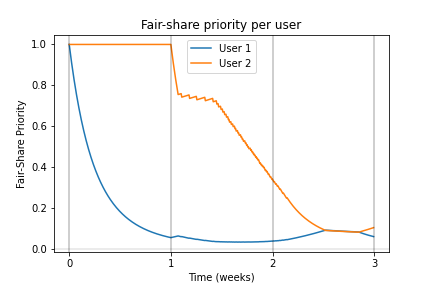
\includegraphics[width=0.8\textwidth]{sim-2-fairshare}
  \end{center}
  \caption{Run 2: Fair-share factor for each user.
    \label{fig:two-fs}}
\end{figure}


\section{Conclusions}

I think we should increase the \code{PriorityWeightFairShare} factor
to at least \code{10000}.  We \emph{may} want to decrease the
\code{PriorityMaxAge} so that jobs max out their Age priority
accumulation sooner.  If we do that, we may want to decrease the
\code{PriorityWeightAge} factor so that jobs accumulate the same
$1000$ priority points per day.

\end{document}
